\documentclass[11pt, a4paper]{report}
\usepackage{graphicx}
\usepackage[table,xcdraw]{xcolor}
\usepackage{geometry}
\usepackage{float}
\usepackage{authblk}
\usepackage{anyfontsize}
\usepackage[document]{ragged2e}
\usepackage{titlesec}
\usepackage[parfill]{parskip}
\usepackage{color}   %May be necessary if you want to color links
\usepackage{hyperref}
\usepackage{caption}
\usepackage{longtable}
\usepackage{blindtext}
\usepackage{pdfpages}
\usepackage[backend=biber]{biblatex}
\hypersetup{
    colorlinks=true, %set true if you want colored links
    linktoc=all,     %set to all if you want both sections and subsections linked
    linkcolor=black,  %choose some color if you want links to stand out
}
\titleformat{\chapter}[hang]
{\normalfont\huge\bfseries}{\chaptertitlename\ \thechapter}{1em}{} 
\geometry{left=2.5cm,right=2.5cm,top=2.5cm,bottom=2.5cm}
\graphicspath{ {./images/} }

\begin{document}  

\pagestyle{empty}
\centering
\fontsize{2cm}{2cm}\selectfont{Module Design Document} \\
\vspace{2mm}
\fontsize{1cm}{1cm}\selectfont Audio digital signal processor \\
\vspace{2mm}
\large BeCreative Minor\\
\normalsize
\vspace{4cm}
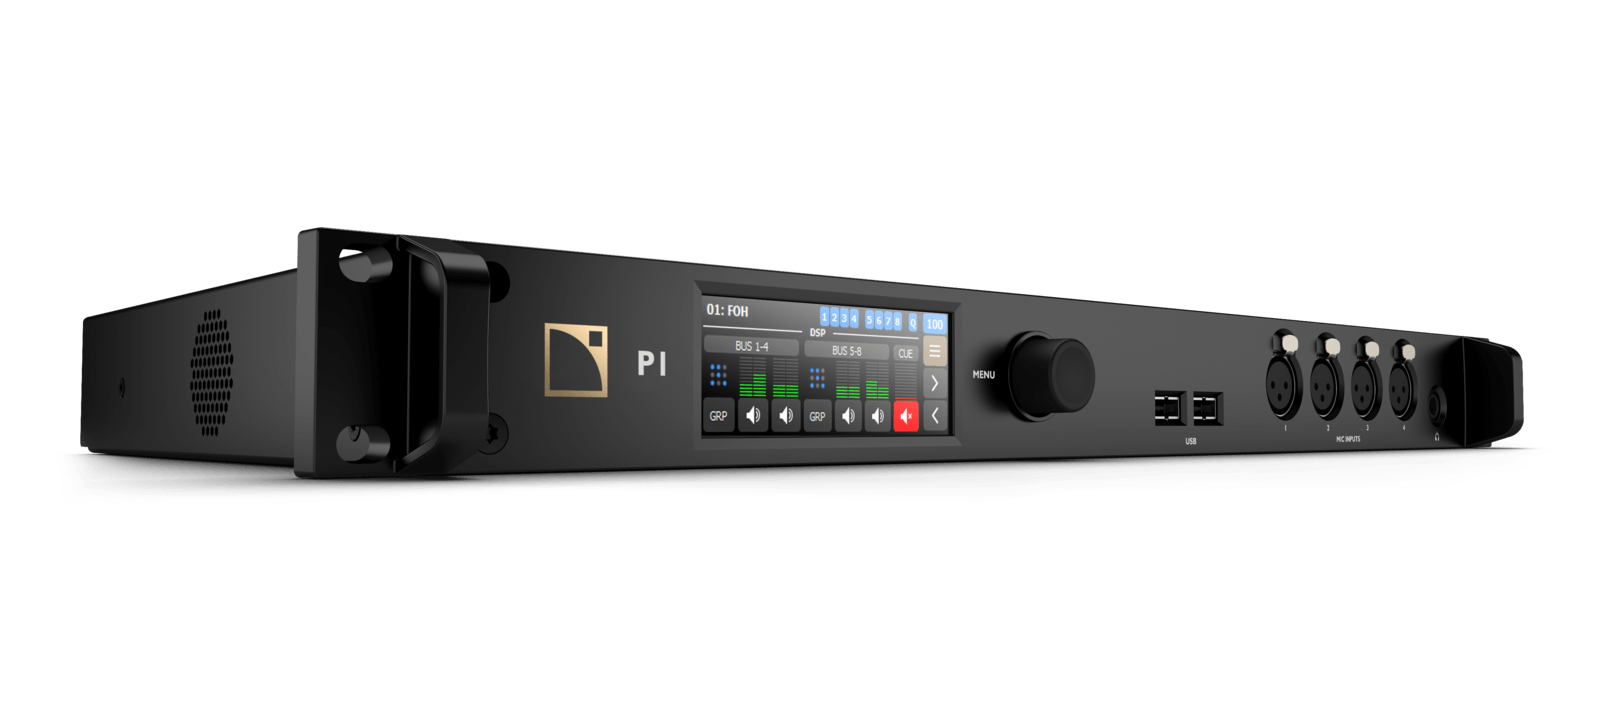
\includegraphics[width=\linewidth]{3DR_P1_Perspective.png}\\
\vfill
\normalsize Busse Lommers \\
Robin van den Dungen \\
Mahmud Gürler \\
Silas Kamphuis \\
Hein Verhallen \\
Youri Tils \\
Fontys Hogescholen, De Rondom 1, 5612 AP Eindhoven \\
\today

\begin{justify}

%\chapter*{Summary}

\newpage
\tableofcontents
\thispagestyle{empty}

\listoffigures
\thispagestyle{empty}


\listoftables
\thispagestyle{empty}

\newpage
\pagestyle{plain}
\setcounter{page}{1}

\chapter*{Abbreviation List}

\begin{table}[!h]
	\centering
\begin{tabular}{|c|c|}
	\hline
\textbf{Abbreviation} & \textbf{Explanation}        \\ \hline
DSP 					& Digital Signal Processor    \\ \hline
ADC 					& Analog-to-Digital Converter \\ \hline
DAC 					& Digital-to-Analog Converter \\ \hline
RAM 					& Random access memory	    \\ \hline
SINAD 					& Signal to noise and distortion \\ \hline
TRS 					& Tip ring sleeve connector (jack) \\ \hline
FPGA 					& Field programmable gate array \\ \hline
CH 						& Channel					\\ \hline

\end{tabular}
\caption{List of commonly used Abbreviations}
\label{Abbreviation list}
\end{table}


    %\pagestyle{empty}
\centering
\fontsize{2cm}{2cm}\selectfont{Module Design Document} \\
\vspace{2mm}
\fontsize{1cm}{1cm}\selectfont Audio digital signal processor \\
\vspace{2mm}
\large BeCreative Minor\\
\normalsize
\vspace{4cm}
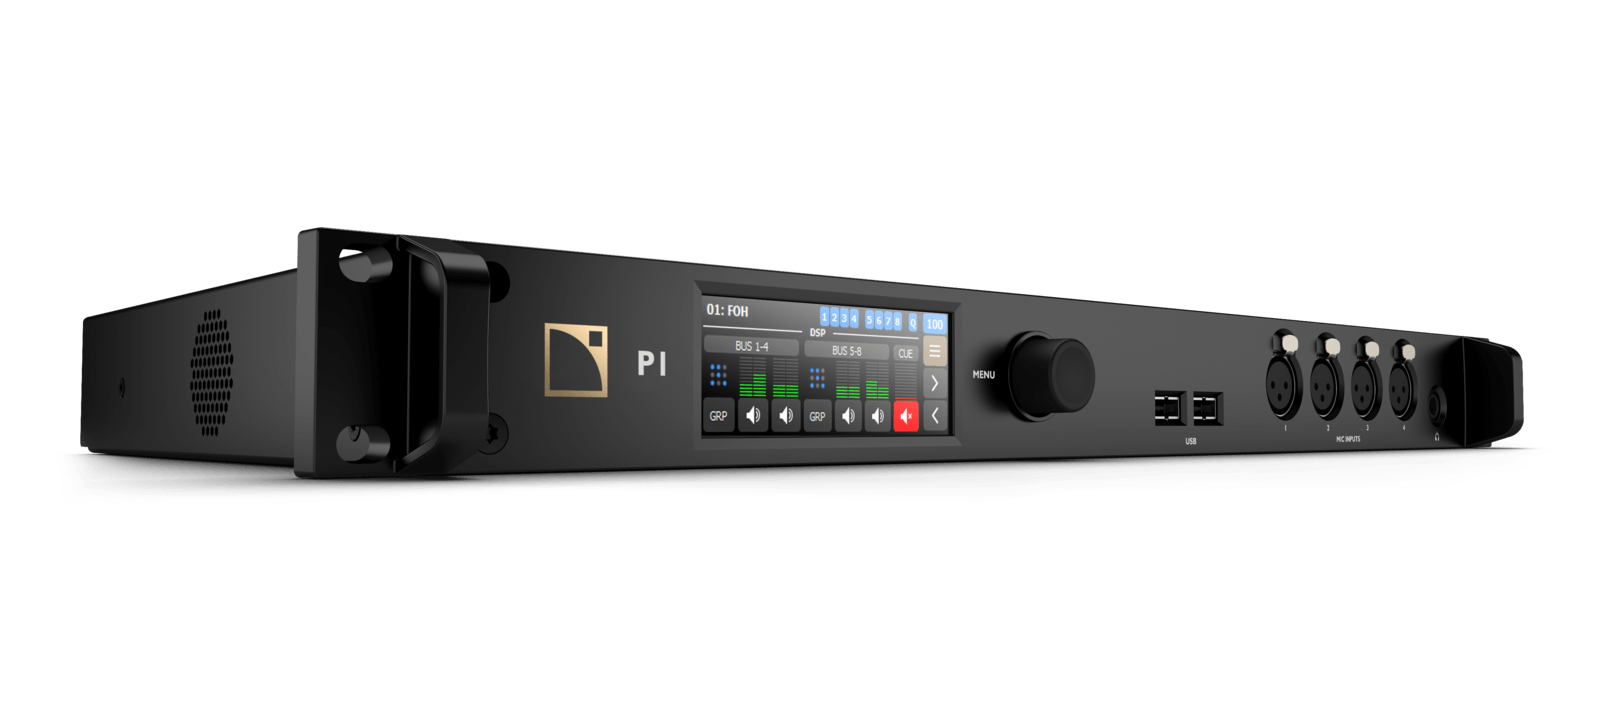
\includegraphics[width=\linewidth]{3DR_P1_Perspective.png}\\
\vfill
\normalsize Busse Lommers \\
Robin van den Dungen \\
Mahmud Gürler \\
Silas Kamphuis \\
Hein Verhallen \\
Youri Tils \\
Fontys Hogescholen, De Rondom 1, 5612 AP Eindhoven \\
\today

\begin{justify}

\chapter*{Summary}
The following text translates to English as:

This report describes how this project group created an audio DSP for the BeCreative Minor. This was done because the members of the group wanted to learn more about it and improve their technical knowledge.

Chapter "Problem Description" outlines the project's background and goals. Chapter "Research" describes the preliminary investigations conducted. Chapter "Concept Development" explains how the product concept was developed. Chapter "Realization" details the actual design of the audio DSP. Chapter "Verification" discusses the product testing process. Finally, in chapters "Conclusions" and "Recommendations," the conclusion and recommendations are respectively described.

\newpage
\tableofcontents
\thispagestyle{empty}

\listoffigures
\thispagestyle{empty}

\listoftables
\thispagestyle{empty}

\newpage
\pagestyle{plain}

\chapter*{Report contribution}	%Fill-in only regarding the report contribution.
\begin{longtable}{|c|c|c|}
	\hline
	\textbf{Chapter} & \textbf{Paragraph} & \textbf{Person} \\ \hline
	Problem Description			& Background					& All	 					\\ \hline
	Introduction				& NA							& Busse 					\\ \hline
								& Problem description			& Robin						\\ \hline
								& Project goals					& All						\\ \hline
								& Requirements					& All 						\\ \hline
								& Project scope					& All 						\\ \hline
								& Boundary condition			& All						\\ \hline
								& Project approach				& All						\\ \hline
								& Verification method			& All						\\ \hline
	Research 					& Research objectives			& All 						\\ \hline
								& Research questions			& All 						\\ \hline
								& Research approach				& All 						\\ \hline
								& Results						& All 						\\ \hline
	Concept Development 		& Concept overview				& Youri						\\ \hline
								& Front-end						& Silas						\\ \hline
								& Audio-DSP						& Youri						\\ \hline
								& Back-end						& Silas						\\ \hline
								& Interfacing					& Robin						\\ \hline
								& Front-end						& Robin						\\ \hline
								& Audio-DSP						& Youri						\\ \hline
								& Back-end						& Robin						\\ \hline
								& Power supplies				& Mahmud \& Robin			\\ \hline
								& Modules						& Busse						\\ \hline
								& UI							& Hein \& Busse				\\ \hline
								& Hardware programming			& Busse						\\ \hline
								& Hardware design				& Busse						\\ \hline
								& Design decissions				& Busse						\\ \hline
	Realization					& Hardware						& NA						\\ \hline
								& Schematic						& Robin						\\ \hline
								& Printed circuit board			& Silas						\\ \hline
								& Case							& Busse						\\ \hline
								& Firmware						& Youri						\\ \hline
								& I2S decoder and encoder		& Youri						\\ \hline
								& I2C controller				& Youri						\\ \hline
								& Band-pass filter				& Youri						\\ \hline
								& Sinewave generator			& Youri						\\ \hline
								& Effects						& Youri \& Busse			\\ \hline
								& User interface				& Hein \& Busse				\\ \hline
								& User interface				& Hein \& Busse				\\ \hline
	Verification				& Method						& Robin						\\ \hline
								& Hardware						& Mahmud \& Robin			\\ \hline
								& Firmware						& Youri						\\ \hline
								& Results						& NA						\\ \hline
								& Hardware						& Mahmud					\\ \hline
								& Firmware						& Youri						\\ \hline
								& Conclusions					& Mahmud \& Silas \& Robin 	\\ \hline
								& Hardware						& Mahmud					\\ \hline
								& Firmware						& Youri						\\ \hline
	Conclusions					& NA							& Silas						\\ \hline
	Recommendations				& NA							& Silas						\\ \hline
	Summary						& NA							& Robin						\\ \hline
	Bibliography				& NA							& Busse						\\ \hline
	Appendix A: State-space		& NA							& Youri						\\ \hline
	Appendix B: VHDL code		& I2S decoder					& Youri						\\ \hline
								& I2S encoder					& Youri						\\ \hline
								& I2C master					& Youri						\\ \hline
								& State-space BPF code			& Youri						\\ \hline
								& Sinewave generator code		& Youri						\\ \hline
	Appendix C: Schematics		& Buck converter schematic		& Mahmud					\\ \hline
								& SEPIC schematic				& Silas						\\ \hline
								& Linear regulator schematic	& Silas	\& Robin			\\ \hline
								& Main board schematic			& Robin						\\ \hline
								& Buck converter calculations	& Silas						\\ \hline
								& SEPIC calculations			& Robin						\\ \hline
	Appendix D: UI design		& Main menu						& Busse						\\ \hline
								& Adjust preset menu			& Busse						\\ \hline
	Appendix E: Case			& Top view						& Busse						\\ \hline
								& Front view					& Busse						\\ \hline
								& Rear view						& Busse						\\ \hline
	Appendix F: Verification	& Ground spring					& Robin						\\ \hline

	\caption{Revision list of the document}
	\label{table:revision_history}
\end{longtable}

\newpage
\pagestyle{plain}
\setcounter{page}{1}

\chapter*{Abbreviation List}

\begin{table}[!h]
	\centering
	\begin{tabular}{|c|c|}
		\hline
		\textbf{Abbreviation} & \textbf{Explanation}	\\ \hline
		DSP 					& Digital Signal Processor    				\\ \hline
		ADC 					& Analog-to-Digital Converter 				\\ \hline
		BPF 					& Band-Pass Filter							\\ \hline
		CH 						& Channel									\\ \hline
		DAC 					& Digital-to-Analog Converter 				\\ \hline
		FFT 					& Fast Fourier Transform					\\ \hline
		FPGA 					& Field programmable gate array 			\\ \hline
		GBW 					& Gain Bandwidth Product 					\\ \hline
		RAM 					& Random Access Memory	    				\\ \hline
		SEPIC        			& Single-Ended Primary-Inductor Converter	\\ \hline
		SINAD 					& Signal to noise and distortion 			\\ \hline
		TRS 					& Tip ring sleeve connector (jack) 			\\ \hline
	\end{tabular}
	\caption{List of commonly used Abbreviations}
	\label{table:Abbreviation list}
\end{table}

    \chapter{Introduction}
    The aim of this project was to fully develop an audio digital signal processor. During the project we researched and developed what it takes to make a working digital signal processor with a custom PCB and an FPGA-board. To house this we researched the ideal layout of the circuit boards and ports. 
\par
\noindent This paper shows the research and design process of the audio digital signal processor. It should contain the needed information to understand what was needed to visualize and create this product. 
Using our skills as engineering students we tried to develop an audio digital signal processor that has enhanced processing capabilities of audio, and is user-friendly and intuitive to use. 


    \chapter{Problem description}
    \section{Background}
%BACKGROUND

\noindent In the audio realm, digital signal processors (DSP) are employed to optimize sound systems. Since perfect speakers do not exist, all speakers inherently possess certain imperfections. However, a DSP can compensate for these imperfections and provide corrective measures. Additionally, DSPs are frequently utilized to enhance the dynamics of sound and imbue it with a distinct character or sensation.

\noindent As a group, we have chosen to develop an audio DSP for the BeCreative minor because we are eager to learn how audio DSPs function and how to create one ourselves. Our ultimate goal is to be able to utilize this audio DSP to enhance the listening experience of music by correcting for speaker imperfections and applying specific presets. The system must meet the requirements outlined in the System Requirements Document (SRD), but what is most important to us is the opportunity for learning and acquiring valuable knowledge throughout the process.


\section{Problem description}

\noindent When it comes to listening to music, it is crucial that the speakers are appropriately calibrated to both the surrounding environment and the position of the listener. This calibration is essential in order to achieve the best possible listening experience since sound pressure varies depending on the frequency at specific locations, characterized by nodes and antinodes. These nodes and antinodes shift throughout the space depending on the frequency. As a high fidelity (Hi-Fi) music listener, it is desirable to have the sound from all speakers reach you simultaneously. However, speakers are often not optimally positioned due to certain physical characteristics of the room. In cases where the speakers are not properly aligned with the surrounding environment, a digital signal processor can be utilized to rectify this issue. A DSP is a specialized processor designed specifically for digital signal processing.

\section{Project goals}

The goal of this project was to research how to make an audio-DSP. This raised the main research question: \textbf{“How to design an audio-DSP?”}. In the process of researching this an actual audio-DSP has been developed. From the main research question the following sub-research questions were derived:
\begin{itemize} %THIS IS TO MAKE LISTS
	\setlength\itemsep{-0.3em} %MAKES THE GAP SMALLER BETWEEN 2 ITEMS
	\item What is the best method for creating digital filters?
	\item What is the best method for creating digital effects?
	\item What is the most suitable anti-aliasing filter?
	\item What is the optimal needed roll-off for the anti-aliasing filter for a given bandwidth such that the noise can be negligible?
	\item What is the minimum sample frequency needed to capture the desired frequency spectrum?
	\item What is the minimum frequency range to be sampled to achieve sufficient detailed audio?
	\item What is the lowest allowable noise for decent audio?
	\item What analog to digital converter (ADC) resolution is needed such that the quantization error and noise level are on par?
	\item What ADC and digital to analog converter (DAC) architecture is most suitable for this application?
	\item What kind of processor is most suitable for this application?
	\item What is the permittable jitter for accurate audio?
	\item What is the maximum allowable ripple on the reference voltage for the ADC and DAC?
	\item How much RAM does the system need?
	\item How much flash does the system need?
	\item What power supply topology is best suited for each part of the system?
\end{itemize}



\par
\noindent
The audio system has some requirements to specify the final result. These requirements are derived with the “MoSCoW” method. It must be noted that the following requirements will be confirmed by the research that will be conducted.

	\newpage
	\section{Requirements}
	\begin{longtable}{|c|p{10cm}|c|c|}
		\hline
		\textbf{ID} & \textbf{Requirement} & \textbf{Priority} & \textbf{Status}\\ \hline 
		\textbf{U1} & \textbf{Inputs:} \newline
		•Two RCA audio inputs which work on a line level of 4dBu(±1,74V)\newline
		•Two 6,35mm TRS plug audio inputs which work on a line level of 4dBu(±1,74V)\newline
		•Two XLR audio inputs which work on a line level of 22dBu(±9,75)\newline
		•USB type B audio input & Must & Proposed\\ \hline

		\textbf{U2} & \textbf{Outputs:} \newline
		•Two RCA audio outputs which work on a line level of 4dBu(±1,74V)\newline
		•Two 6,35mm TRS plug audio outputs which work on a line level of 4dBu(±1,74V)\newline
		•Four XLR signal outputs which work on a line level of 22dBu(±9,75)
		 & Must & Proposed\\ \hline

		\textbf{U3} &The system should have a bandwidth (±3 dB) of at least 20 Hz up and till 20 kHz without any filters applied. 	& Must   & Proposed\\ \hline
		\textbf{U4} &The system has an Audio sample rate of at least 44.1 kHz 														& Must   & Proposed\\ \hline
		\textbf{U5} &The ADC and DAC resolution is at least 16-bit 																	& Must   & Proposed\\ \hline
		\textbf{U6} &The system has a propagation delay of less than 100ms without any filters applied 								& Must   & Proposed\\ \hline
		\textbf{U7} &User can select what input will be used via a user interface													& Must   & Proposed\\ \hline
		\textbf{U8} &User can select up to 4 effects to active on one channel at the same time 										& Must   & Proposed\\ \hline
		\textbf{U9} &User can configure each effect 																				& Must   & Proposed\\ \hline
		\textbf{U10} &The system must work stand alone and be configurable via a basic graphical user interface 					& Must   & Proposed\\ \hline
		\textbf{U11} &Effects are configurable per output channel, at least four different sound effects should be able to be applied to each signal output signal at the same time: \newline
		\begin{itemize}
			\setlength\itemsep{-0.4em}
			\item Distortion
			\item Reverb
			\item Gain
			\item Equalizer
			\item Delay
		\end{itemize}																												& Must 	 & Proposed\\ \hline
		\textbf{U12}  &The system should have a bandwidth (±1 dB) of at least 20 Hz up and till 20 kHz without any filters applied 	& Should & Proposed\\ \hline
		\textbf{U13}  &Audio sample rate of at least 96 kHz 																		& Should & Proposed\\ \hline
		\textbf{U14} & The ADC and DAC resolution is at least 24-bit. 																& Should & Proposed\\ \hline
		\textbf{U15} & Six XLR signal outputs work on a line level of 22 dBu (±9,75 V) 												& Should & Proposed\\ \hline
		\textbf{U16} & User can select up to 10 effects to be active in one channel at the same time. 								& Should & Proposed\\ \hline
		\textbf{U17} & Low enough jitter to not influence the audio quality too much 												& Should & Proposed\\ \hline
		\textbf{U18} & Local power supplies for different parts of the system 														& Should & Proposed\\ \hline
		\textbf{U19} & Low enough jitter to not influence the audio quality too much 												& Should & Proposed\\ \hline
		\textbf{U20} & Effects:\newline
		\begin{itemize}
			\setlength\itemsep{-0.3em}
			\item Phaser
			\item Tremelo
			\item Flanger
			\item Fuzz
			\item Overdrive
			\item Chorus
			\item Compressor
			\item Wah
			\item Looper
			\item Wow and flutter
			\item Modulator
			\item Echo
			\item Fade in
		\end{itemize}																												& Should & Proposed\\ \hline
		\textbf{U21} & Audio sample rate of at least 192 kHz 																		& Could  & Proposed\\ \hline
		\textbf{U22} & Touch screen user interface 																					& Could  & Proposed\\ \hline
		\textbf{U23} & Self-made mains power supply  																				& Won't  & Proposed\\ \hline
	\end{longtable}

\section{Project scope}

The project is conducted during the minor BeCreative at Fontys. This minor took 20 weeks and allowed the students to have a budget of €300,-. Thus after 20 weeks starting from 6-2-2023 an audio-DSP has been delivered within a budget of €300,-.
\par 
\noindent Weekly meetings were conducted with the project's assessor to keep the research and tasks on track, and to ask questions regarding specific things about the hardware or firmware. 

\section{Boundary condition}

The needed mains power supply will not be made during this project and will be bought externally.

\noindent For the power supply a transformer is used to make a safe voltage.


\section{Project approach}

The project is guided by a system of dividing tasks, having weekly meetings, and keeping each other up-to-date by asking questions outside of meetings. Research is divided and cohering tasks are assigned. To keep track of what has to be done, a planner has been made to see when certain tasks need to be done.

\section{Verification method}

At the end of the semester there should be a working audio DSP capable of the must-have requirements. 



    \chapter{Research}
    \section{Research objectives}

\section{Research questions}

\section{Research approach}

\section{Results}

\section{Conclusions}



    \chapter{Concept Development}
    \section{Concept overview}

\section{Architecture}

\section{Block diagrams}

\section{Modules}

\section{Design decisions}




    \chapter{Realization}
    \section{Hardware}

\subsection{Case}
To house all the components that make the DSP, a 19 inch 2U rack case is used. These cases are used for a lot of audio processing devices. This makes it easier to keep a system organized. The DSP fits nicely into an existing audio rack somebody may use.
\par 
\noindent The case is fitted with all the needed ports on the back, a screen and knob in the front left, and 16 LEDs for showing VU-readings in the front right. Power is connected via a metal female DC connector so that, when not in use, the case has no wires attached. 
\par
\noindent Mounted inside the case is an FPGA-board and a custom PCB loaded with all the needed converters. The FPGA-board and PCB are mounted on metal spacers connected to the case with screws. This way of mounting the components was chosen to have a sturdy, robust product.

\section{Firmware}

\section{Software}

\section{User interface}

A well-designed user interface is a critical component of any audio DSP project, particularly when utilizing a Nextion or similar screen. The user interface should be designed with simplicity in mind to ensure it is accessible to everyone who uses it. One of the primary goals of a good UI is to ensure that it is intuitive and easy to remember, so that users can begin using the product without feeling frustrated or overwhelmed.

\subsubsection*{Consistent}
The UI should maintain a consistent style throughout, so that each new menu or dial looks and feels the same as every other menu. This ensures that using the menus is easy and recognizable, even for new users.

\subsubsection*{Readability}
Text shown in menus should not be cut off, as this can be frustrating for users trying to read it. Short sentences are preferred to keep the menus clean and easy to read. When a sentence is cut off by the edge of the screen, users may struggle to figure out what it says, leading to confusion and frustration.

\subsubsection*{Feedback}
Finally, it is important to provide feedback to the user when the system needs time to load in certain elements or execute specific settings. Without feedback, users may become frustrated and begin clicking buttons multiple times, which can lead to software errors. By providing clear feedback during loading processes, users are more likely to remain patient and avoid potential issues.

\subsection{Designing the UI}
The design was started with a diagram with all the necessary screens and information so that is was clear what menus should be in the DSP. 

\begin{figure}[ht]
    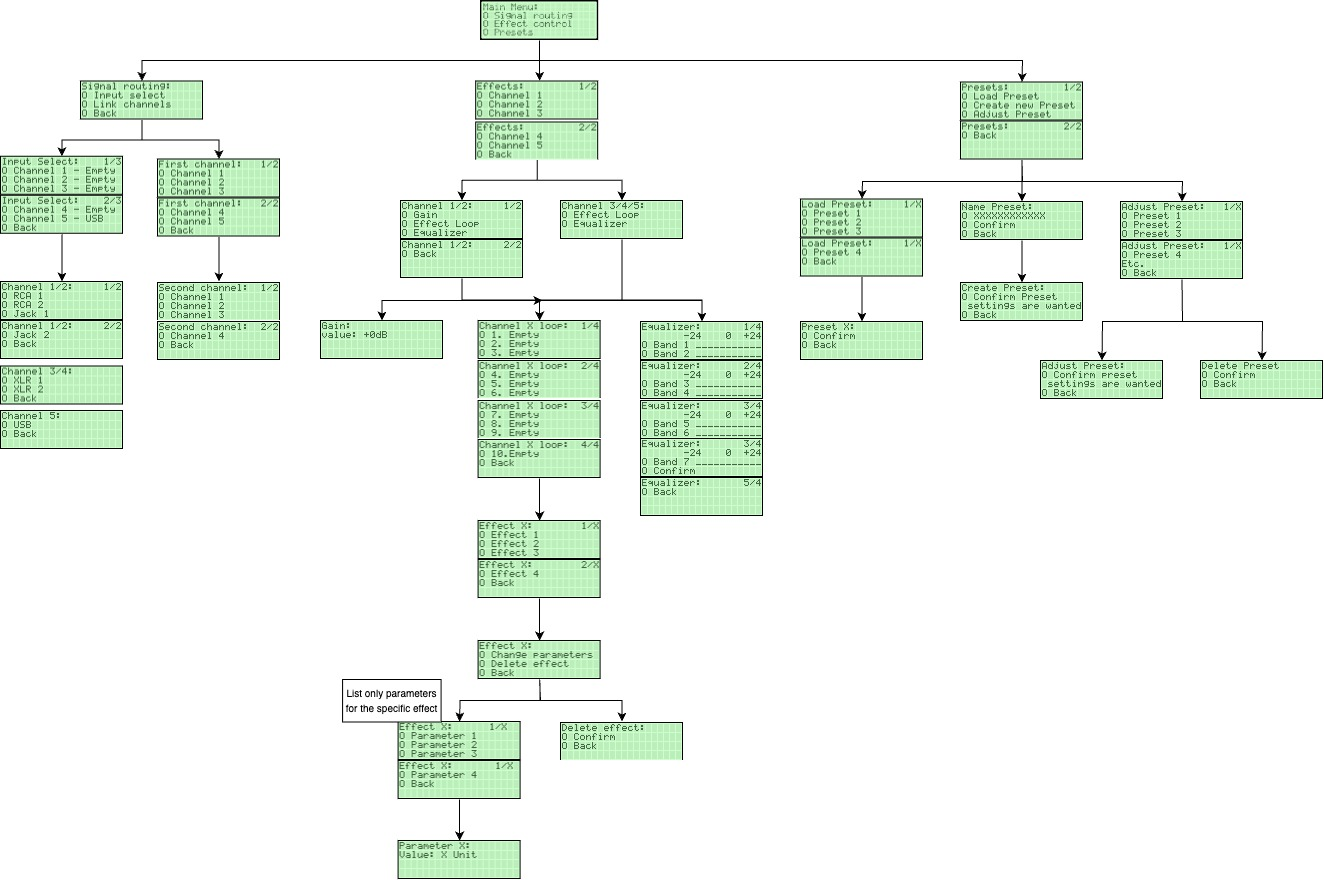
\includegraphics[width=\linewidth]{functionbasedUI}
    \caption{Function Based UI Design for a liquidCrystal screen}
    \label{fig:functionbasedUI}
\end{figure}

This UI is easy to understand when first using the DSP. Options and settings are easy to find from the first menu screen. While a channel based UI is unclear because every option is branched off from the channel select.

\section{Nextion screen}

For this project a Nextion screen is used. This screen can easily be programmed. It comes with software which is image based instead of code based. Images can be inserted and "invisible" buttons can be used to make menus out of the inserted images.

This is a neat way to work because now it is possible to create images in Photoshop or a similar application to use for the whole menu design.

    \chapter{Verification}
    \section{Method}
Time has not yet allowed for the creation of a neat and detailed test plan. However, before the voltage regulator boards are soldered onto the main board, they need to be thoroughly tested to verify their functionality. The plan is to create a test table for this purpose, similar to the specification of ICs in datasheets.

\subsection{Hardware}
\subsubsection{Voltage regulators}
For the voltage regulator modules, the following parameters need to be measured to demonstrate proper operation:
-Thorough visual inspection, especially focusing on the soldering process. This includes checking for short circuits, open connections, solder balls, and other defects.
-The converter should be powered from a lab power supply with low current limit settings. In case of a short circuit or other module defect, the dissipated power will be limited, allowing for the identification and resolution of the issue.
-The output voltage of the converter should be observed using an oscilloscope. Attention should be paid to the absolute accuracy and the amplitude of the ripple voltage.
-The temperature of the PCBA should be monitored to ensure that the module does not get too hot, which could potentially shorten its lifespan.

\subsubsection{Main board}
The functionality of the main board should be verified in the following manner:
-Perform a thorough visual inspection, with a focus on the soldering process. Check for short circuits, open connections, solder balls, and other defects.
-Power the main board from a lab power supply with low current limit settings. This will limit the dissipated power in case of a short circuit or module defect, enabling identification and resolution of the issue. A thermal camera can be used to inspect the PCBA for hotspots.
-Verify the presence and correctness of all power rails.
-Verify that the output of the GPIO pins corresponds to the desired outcome.(e.g. check the SLCK).
-Next, apply a known signal (e.g., a 1kHz sinusoidal waveform with an amplitude of 100mV) to the various inputs of the audio-DSP. If no filters are selected and the audio-DSP is essentially in a pass-through state, the same signal should appear on the selected outputs. The accuracy of this signal can be verified using an audio analyzer such as the AP SYS 2700.

\subsection{Firmware}
The firmware can be tested by simulating the VHDL code in Modelsim. For this .do files are made to force input signals. Due to time constrains only the I2S decoder and encoder have been tested with real audio. 

\subsubsection{I2S decoder and encoder}
For testing the I2S decoder and encoder, they are wired in series. So when a random data pattern is going in the decoder the encoder should output the same data pattern.

\subsubsection{I2C master}
The I2C master is tested by simply writing and reading data with the protocol and verifying that the protocol works correctly according to the I2C protocol standards. 

\subsubsection{State-space BPF}
The state-space BPF is tested by inputting a sine wave outputted from a sine wave generator. By using a sine wave as an input it is very easy to expect the outcome. For instance when having the BPF resonance frequency at 1kHz and inputting a 1kHz sine wave, it is expected that the output sine wave has the same amplitude compared to the input sine wave. And when the frequency of the input sine wave does not match that of the BPF resonance frequency, it will be attenuated. 

The best way to check if the band-pass filter works is by changing the frequency of the input sine wave over time to create a kind of frequency spectrum of the band-pass filter response. 

\subsubsection{Effects}
All the effects are tested by inputting a sine wave to the effect and looking at the result. This approach with a simple sine wave input is chosen because with a sine wave input it is very simple to predict the outcome of the effect and then confirm if it works as expected.

\section{Results}

\subsection{Hardware}

\subsubsection{Buck}
Due to the limited time, this verification has not been done yet.

\subsubsection{Linear voltage regulator}
After conducting a thorough visual inspection, it became apparent that a thorough cleaning of the PCBA was necessary. This was because the solder paste used left behind a significant amount of residue. Therefore, the linear voltage regulators were cleaned in an ultrasonic cleaner.

Subsequently, the linear regulators were connected to a lab power supply with current limiting. However, it quickly became evident that the regulators were not functioning properly. After performing several simulations in LTspice, it was suspected that the LEDs, which serve as low-noise voltage references, might have been soldered incorrectly. However, after consulting the datasheet again with several group members, it was confirmed that the LEDs were indeed soldered correctly according to the datasheet.

Since no other plausible causes emerged after further investigation, it was decided to desolder one of the LEDs and measure it out of circuit using a multimeter to determine its polarity and threshold voltage. To the astonishment of the group, it was discovered that the Broadcom datasheet for the HSMH-C170 LED did not match the LEDs actually supplied. The polarity marking in the datasheet was the exact opposite of the actual component. It is unknown whether an incorrect batch was delivered or if the datasheet itself is genuinely incorrect.
%https://nl.mouser.com/datasheet/2/678/AV02_0551EN_DS_HSMx_Cxxx_25Mar2022-1827675.pdf

\subsubsection{Main board}
\paragraph{inspection} Before connecting every module together and placing every component on the main board it is indeed ascertain that the board has flux and solder paste residue together with solder balls that can cause short circuits, therefore the PCBA will be cleaned in the ultrasonic bath, before doing this it is important to know which components are suitable for this. The relays and electrolytic capacitors are not suitable for this, therefore they are soldered after cleaning.  visual inspection has been done on the main board and the power delivery modules. In the second visual inspection there are no signs of shorts and the components are connected properly.
\paragraph{Visual inspection} 

Before connecting every module together and placing every component on the main board it is indeed ascertain that the board has flux and solder paste residue together with solder balls that can cause short circuits, therefore the PCBA will be cleaned in the ultrasonic bath, before doing this it is important to know which components are suitable for this. The relays and electrolytic capacitors are not suitable for this, therefore they are soldered after cleaning.  visual inspection has been done on the main board and the power delivery modules. In the second visual inspection there are no signs of shorts and the components are connected properly.

\paragraph{Vertical riser board}
The vertical riser boards have to be tested before placing it on the main board. These have been tested individually on ripple(not for the linear regulators, no equipment available to measure), output voltage and temperature. See \ref{Appendix-Vertical riser boards} Vertical riser boards in chapter \ref{chap:Appendix-Verification} verification for the outcomes. For the Sepic the output ripple is ~5mV and output is -15.11V which is within specs, the temperature is 70°C at 1A which is feasible but if there is more power required an extra fan can be attached to cool the converter more. The buck converters(see \ref{pdf:5V Buck converter} 5V buck - \ref{pdf:15V Buck converter} 15V buck) in the beginning all had an output of ~1v. This was because the feedback resistors were exchanged together. Therefore they had to be exchanged again and the problem is solved. The output voltage of all the buck converters are within spec. The ripple is ~8-10mV which is also within spec range. The temperature of all the buck converters are below 45°C at 1A. The output of the linear regulators (see \ref{pdf:12V linear regulator-1}12V lin reg up and till \ref{pdf:5V linear regulator-2}5V lin reg) are within specs and the temperature is 80°C at 1A, they won't be conducting more current than that so the temp is within spec range.

\paragraph{Main board power}
The PCBA is inspected and no short circuit is detected. The next step is to check all the power modules within the PCBA with current limiting, so that the board will not be catch on fire if there is somehow still a short. This has been done with a power supply limited to 1A. All the power rails are tested and every power delivery module is working properly at the desired voltage. The 12V buck converter that is going to the FPGA is tested separately first with four 33 resistors connected in parallel which will give 1.5A of current at 12V. The buck is still below 50°C. Therefore it is safe to power the fpga with the 12V buck converter

\paragraph{FPGA GPIO}
After doing visual inspection and vertical riser board inspection, it is safe to connect the fpga with the main board using flat cables. Unfortunately after connecting the the main board with the fpga it is stated that it didn't work after connecting the laptop using an RCA-cable to the audio dsp. The first thing that has been checked is the output of the clock going to the mainboard from the fpga. Doing so it has been identified that indeed the clock was not being transmitted correctly via the gpio pins of the DE1-SOC. In figure \ref{fig:Appendix-24.576MHz clock output} 24.576MHz clock output it is clearly visible that the 24.567MHz signal is clearly filtered due to parasitic capacitances in the signal path. Those effecting the paths are the following components Mosfets, diodes and the 47 ohm resistor at the GPIO pins. In figure \ref{fig:Appendix-50MHz clock output} 50MHz clock output is visible that the signal is even more weakened which makes it evident it is due to parasitic capacitances. In figure \ref{fig:Appendix-1MHz clock output} 1MHz clock output it is visible that the rising edge of the clock is already behaving capacitive. To be sure that the underlying issue is on all boards and not specifically on this board we have tested the clock output on another board and unfortunately the outcome is the same.

\subsection{Firmware}
\subsubsection{I2S encoder and decoder}
The results of this test can be found in figure \ref{fig:sim_result_i2s_dec_enc}. These results show that the I2S encoder and decoder work as expected. 

\subsubsection{I2C master}
The results can be seen in figure \ref{fig:sim_result_i2c-master}. In this result it can be seen that the I2C master works as expected according to the protocol standards.

\subsubsection{State-space BPF}
For testing the state-space BPF it is very easy to see if it works by checking the frequency response. For the test a resonance frequency for BPF of 400Hz is chosen. Then the sine wave changes its frequency every 10ms. The frequency start at 25Hz and steps up in octaves. The end frequency is 51200Hz as this is far beyond the range of the sampling frequency. The result of this test is seen in \nameref{chap:appendix-G-simulation-results}. 

As expected, the amplitude of the sine wave at the matching resonance frequency of 400Hz is equal to the input amplitude. And when the frequency goes an octave lesser or higher in frequency the amplitude is $\frac{\sqrt{2}}{2}$ times the input amplitude (-3dB). This is a result that is expected from a BPF, therefore it is shown that the BPF works in simulation.

\subsubsection{Effects}
\paragraph{Volume control}


\section{Conclusions}
\subsection{Hardware}

\subsubsection{Buck}
Due to the limited time, this verification has not been done yet.

\subsubsection{SEPIC}
The SEPIC appears to be functioning well after some quick measurements. With an input voltage of +12V, it generates a stable -15V output voltage, and the voltage ripple remains nearly constant regardless of the output current. This aligns with the calculations and simulations. Additionally, the amplitude of the output ripple voltage closely matches the calculated and simulated values.

\subsubsection{Linear voltage regulator}
Due to the limited time, this verification has not yet been completed.

\subsubsection{Main board}
Due to the limited time, this verification has not been done yet.

\subsection{Firmware}
The I2S decoder, I2S encoder and I2C master work as expected. Therefore it is possible to sample audio using the ADC and DAC of the FPGA board. This has been tested and verified that this works. 

Due to time constrains further testing and implementation of the effects has not been conducted. 


    \chapter{Conclusions}
    Due to time constrains the final project is not yet working. The hardware main board has been tested for as far as possible and works for as far as could be tested. Also all the vertical riser boards have been tested and validated as shown in the verification chapter. The firmware that has been developed for the product has been tested in ModelSim and works there, but still has to be implemented in combination with the hardware. 
\par
<<<<<<< HEAD
\noindent During testing of the DE1-SOC board a problem has been found. The clock signal that goes from the FPGA to the DAC's and ADC's is not working properly. The output of the DE1-SOC FPGA board seems to be to capacitive due to parasitics of the board design and therefore the clock signal gets filtered down and is not picked up by the ADC's and DAC's. The schematic of the FPGA board shows that there is a 47 Ω series resistor, this in combination with the RDS(on) of the internal switching FETs of the Cyclone-V and the capacitance of the TVS diode in parallel with the parasitic capacitance of the PCB seems to cause the clock signal to be filtered out as an Rc-LPF. The measurements where done on the DE1-SOC board that was not connected to the Main board of the DSP to exclude our main board and flat cable from this conclusion.
=======
\noindent During testing of the DE1-SOC board a problem has been found. The clock signal that goes from the FPGA to the DACs and ADCs is not working properly. The output of the DE1-SOC FPGA board seems to be to capacitive due to parasitics of the board design and therefore the clock signal gets filtered down and is not picked up by the ADCs and DACs. The schematic of the FPGA board shows that there is a 47 Ohm series resistor, this in combination with the RDS(on) of the internal switching FETs of the Cyclone-V and the capacitance of the TVS diode in parallel with the parasitic capacitance of the PCB seems to cause the clock signal to be filtered out as an RC-LPF. The measurements where done on the DE1-SOC board that was not connected to the Main board of the DSP to exclude our main board and flat cable from this conclusion.
>>>>>>> 6baa9264baaf424ca591278f70fbd15759b66a8a


    \chapter{Recommendations}
    Due to time constraints the project has not yet been finished. Most parts have been tested and work as expected, but some parts still have to be implemented and tested according to the planning. Some more time is needed to finish the Project.
\par
\noindent The following recommendations have been made to help the project work/ work better:

\begin{itemize}
    \setlength\itemsep{-0.3em} %MAKES THE GAP SMALLER BETWEEN 2 ITEMS
    \item Do not use FFT for the processing, use a direct approach instead or use a way more powerful processor
    \item Look into the clock signals from the FPGA board to the main PCB
    \item Investigate if there are other FPGA boards available which do support the needed 24.576 MHz output frequency on their GPIO pins
    \item Indicate on the UI screen which option is selected
    \item Make a less enthusiastic project planning
\end{itemize}

    \chapter*{References}
    \addcontentsline{toc}{chapter}{References}  

    \chapter*{Appendices}
    \addcontentsline{toc}{chapter}{Appendices}
    Hello World!
    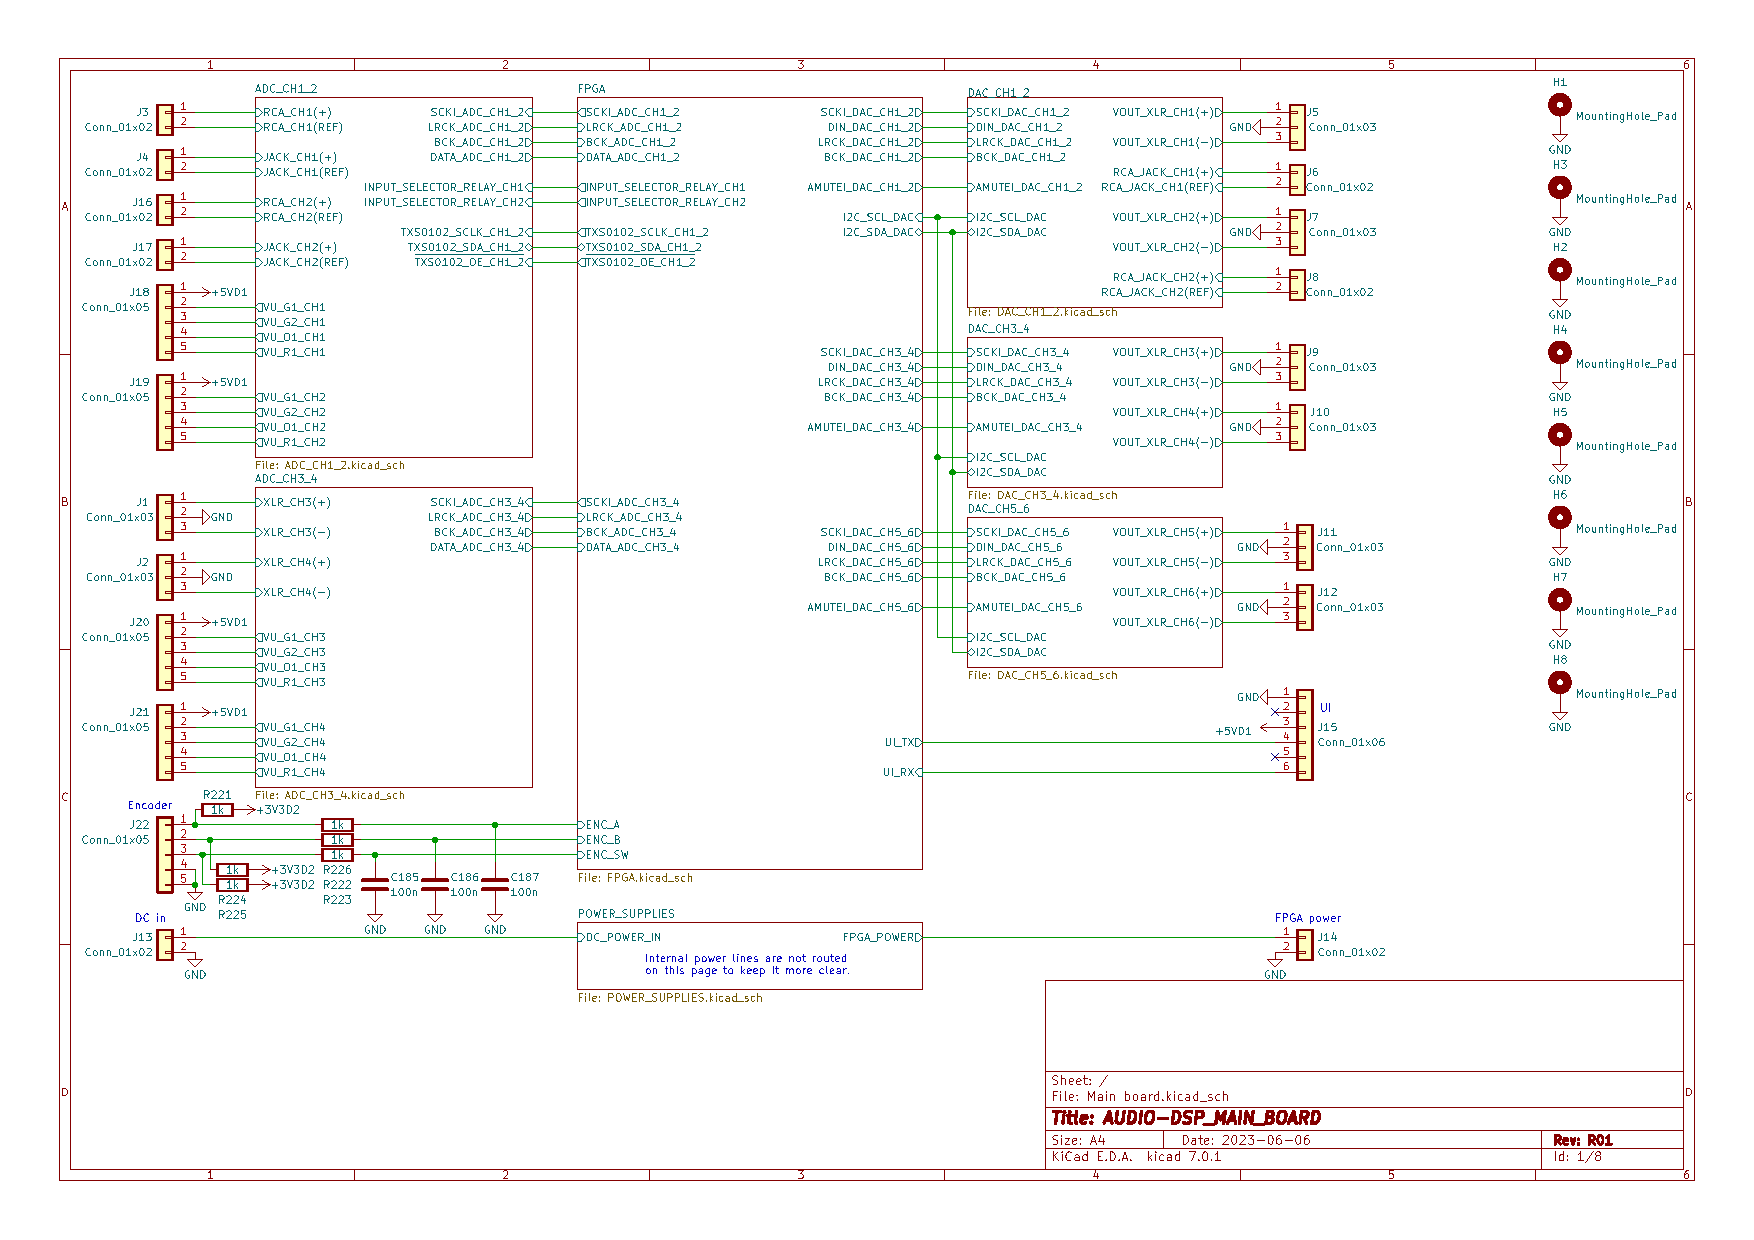
\includepdf[pages=-]{Main_board_schematic.pdf}

    \end{justify}
\end{document}